\documentclass[a4paper,10pt]{article}

\usepackage[latin1]{inputenc}
\usepackage[spanish]{babel}
\usepackage{fontenc}
\usepackage{graphicx}
\usepackage{url}
\usepackage{verbatim}
\author{Nicol\'as Bombau \and Carlos Castro \and Dami\'an Dom\'e \and Emmanuel Teisaire}
\title{Software Design Specification \\ Phyloloc}
\pagestyle{headings}
\begin{document}
\maketitle
\newpage
\tableofcontents
\newpage
\section{Introduction}
  \subsection{Document Purpose}
  
\paragraph{}
The purpose of the current document is the software design specification for the product ``Phyloloc''.

\subsection{Document Audience}
  
\paragraph{}
The intended audience for the current document are the people involved in the thesis and future contributors.

\subsection{Document Organization Overview}

\paragraph{}
Section~\ref{considerations} mentions the objectives of the current document, the design methodology adopted and enumerates design dependencies.

\paragraph{}
Section~\ref{architecture} introduces the system's architecture, and its main components and interactions.

\paragraph{}
Section~\ref{hld} details the system's high level design, presenting the system's packages and interfaces.

\paragraph{}
Section~\ref{lld} specifies the system's low level design, where concrete classes and class diagrams are presented, together with dynamic diagrams, that shall illustrate the system's main processes.

\section{Design Considerations}
\label{considerations}

\subsection{Objectives}

\paragraph{}
The objective in regard to the software design, is the development of a product that presents a concise, mantainable and extensible object oriented design.

\subsection{Design Methodology}

\paragraph{}
The design methodology adopted is ``Responsibility Driven Design''. This technique focuses on \textit{what} responsibilities must be covered by the system, and which objects shall carry those responsibilities.


\subsection{Dependencies}

\paragraph{}
The product shall use Qt for the GUI, and Spirit for text processing in order to work properly. On the other hand, an interface shall be defined, so that the system consumes the methods of the interface, regardless of its implementation, so that the external libraries can be easily changed.


\subsection{Tools}

\begin{itemize}

   \item \textbf{UML} as modelling language.

   \item \textbf{ARGOUML:} as modelling tool.
   
   \item \textbf{Enterprise Architect:} as modelling tool.

   \item \textbf{Gcov and LCov:} to calculate code coverage.
   
   \item \textbf{CCCC:} to calculate code metrics.

   \item \textbf{Doxygen:} to document code. 
   

\end{itemize}

\subsection{Conventions}
\subsubsection{Interfaces}
Interfaces shall be called as their default implementation class name, adding a character ``I'' at the beginning. For example, the interface of the \emph{Person} class, shall be \emph{IPerson}.

\section{System Architecture}
\label{architecture}

\paragraph{}
In this section is discussed and defined the architecture of the system. In Figure~\ref{uml:architecture} is presented a diagram containing the system's architecture, and the interaction between its components. A brief description of each component is presented below:

\subsection{Domain}

\paragraph{Responsibility:} Define the domain model.

\subsection{Phylopp}

\paragraph{Responsibility:} Provide generic primitives for phylogenetic trees, such as Traversals and Tree Consense.
\begin{enumerate}
       \item Domain
      \end{enumerate}
	  
\subsection{Phyloloc}

\paragraph{Responsibility:} Implement the product-specific algorithms that take part in the propagation process.
\paragraph{Collaborators:}
      \begin{enumerate}
       \item Domain
	   \item Phylopp
      \end{enumerate}
	  
\subsection{PhyloGUI}

\paragraph{Responsibility:} Let the user visualize and process phylogenetic trees
\paragraph{Collaborators:}
      \begin{enumerate}
       \item Domain
	   \item Phyloloc
      \end{enumerate}
	  
\subsection{Main}

\paragraph{Responsibility:} Run initialization and configuration tasks.
\paragraph{Collaborators:}
      \begin{enumerate}
	   \item PhyloGUI
      \end{enumerate}
	  

  \begin{figure}
  \centering
  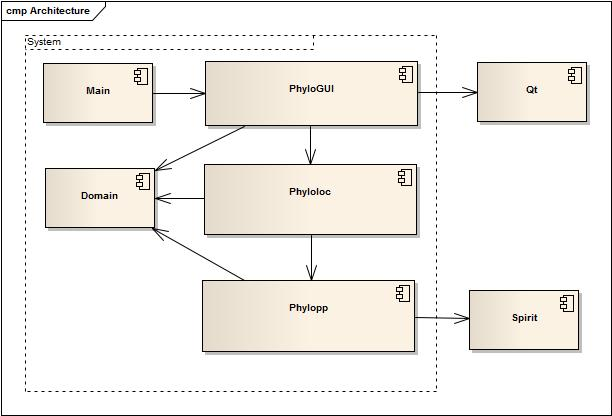
\includegraphics[scale=0.5]{images/Architecture.jpg}  
  \caption{UML - Arquitectura}
  \label{uml:architecture}
  \end{figure}

\section{High Level Design}
\label{hld}

\subsection{Packages}

\paragraph{}
The packages detailed below were identified by analyzing the responsibilities of each component, and afterwards grouping those responsibilities in packages.

In Figure~\ref{uml:packages} is presented a diagram containing the packages and relations between them.

  \begin{figure}
  \centering
  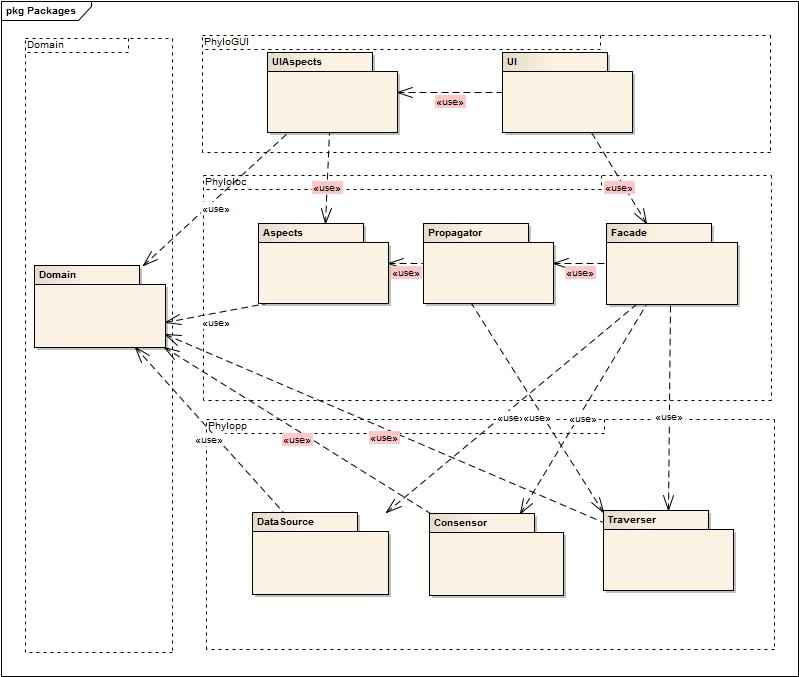
\includegraphics[scale=0.5]{images/Packages.jpg}  
  \caption{UML - Paquetes}
  \label{uml:packages}
  \end{figure}

\subsubsection{Domain}

\paragraph{Responsibility:} Represent the objects of the domain model, such as nodes, trees and groups of phylogenetic trees.

\subsubsection{Consensor}

\paragraph{Responsibility:} Consense a collection of phylogenetic trees, obtaining a single tree. The Consense algorithm to implement must be a Strict Consense algorithm.
\paragraph{Collaborators:}
      \begin{enumerate}
       \item Domain
      \end{enumerate}

\subsubsection{Traverser}

\paragraph{Responsibility:} Provide simple ways to traverse phylogenetic trees from tips to root and from root to tips.
\paragraph{Collaborators:}
      \begin{enumerate}
       \item Domain
      \end{enumerate}

\subsubsection{DataSource}

\paragraph{Responsibility:} Import and export phylogenetic trees.
\paragraph{Collaborators:}
      \begin{enumerate}
       \item Domain
      \end{enumerate}

\subsubsection{Propagator}

\paragraph{Responsibility:} Propagate probabilities through a phylogenetic tree in order to integrate topological and geographical data.
\paragraph{Collaborators:}
      \begin{enumerate}
       \item Traverser
      \end{enumerate}

	  \paragraph{Responsibility:} Provide application-specific aspects for a node, like propagation and consense information.
\paragraph{Collaborators:}
      \begin{enumerate}
       \item Domain
      \end{enumerate}
	  
\subsubsection{Facade}

\paragraph{Responsibility:} Provide a common interface or set of interfaces in order to simplify the integration with other systems or user interfaces.
\paragraph{Collaborators:}
      \begin{enumerate}
       \item Propagator
       \item Consensor
       \item Traverser
      \end{enumerate}
	  
	  \subsubsection{UI}

\paragraph{Responsibility:} Control the data to be displayed and perform the requested operations.
\paragraph{Collaborators:}
      \begin{enumerate}
       \item Facade
      \end{enumerate}
	  
	  \subsubsection{UIAspects}

\paragraph{Responsibility:} Define aspects for a node, in order to hold information about presentational properties, such as color and selection state.
	  \paragraph{Collaborators:}
      \begin{enumerate}
       \item Aspects
      \end{enumerate}
	  
	  \subsubsection{Aspects}

\paragraph{Responsibility:} Provide application-specific aspects for a node, like propagation and consense information.
\paragraph{Collaborators:}
      \begin{enumerate}
       \item Domain
      \end{enumerate}


\subsection{Interfaces, Responsibilities and Collaborations}

\paragraph{}
In this section shall be presented the system's main interfaces, describing its responsibilities and collaborators. 

  \subsubsection{IIterator}
    \paragraph{Responsibility:} Provide interface to iterate through collections.

  \subsubsection{INode}
    \paragraph{Responsibility:} Hold topological information and basic data associated to a node of a phylogenetic tree.
    \paragraph{Collaborators:}
      \begin{enumerate}
       \item IIterator
      \end{enumerate}
	  
	    
	\subsubsection{INodeFactory}
    \paragraph{Responsibility:} Create node with certain definite aspects
    \paragraph{Collaborators:}
      \begin{enumerate}
       \item INode
      \end{enumerate}

  \subsubsection{ITree}
    \paragraph{Responsibility:} Represent a phylogenetic tree.
    \paragraph{Collaborators:}
      \begin{enumerate}
       \item INode
       \item IIterator
      \end{enumerate}

  \subsubsection{ITreeCollection}
    \paragraph{Responsibility:} Represent a collection of phylogenetic trees.
    \paragraph{Collaborators:}
      \begin{enumerate}
       \item INode
       \item IIterator
      \end{enumerate}

  \subsubsection{IDataSourceInfo}
    \paragraph{Responsibility:} Provide the information needed in order to access a particular data source.

  \subsubsection{IDataSource}
    \paragraph{Responsibility:} Export and import phylogenetic trees.
    \paragraph{Collaborators:}
      \begin{enumerate}
       \item IDataSourceInfo
       \item ITreeCollection
      \end{enumerate}

  \subsubsection{INodeVisitor}
    \paragraph{Responsibility:} Encapsulate an action to be executed on a node of a phylogenetic tree.

  \subsubsection{ITraverser}
    \paragraph{Responsibility:} Provide simple way to traverse phylogenetic trees down and up.
    \paragraph{Collaborators:}
      \begin{enumerate}
       \item INodeVisitor
	 \item ITree
	 \item INode
      \end{enumerate}

  \subsubsection{IConsensorObserver}
    \paragraph{Responsibility:} Observe the consense process, and start actions depending on the consense event, for example, when a node is supressed, or consensed.

  \subsubsection{IConsensor}
    \paragraph{Responsibility:} Consense a collection of phylogenetic trees, resulting in a single tree.
    \paragraph{Collaborators:}
      \begin{enumerate}
       \item IConsensorObserver
	 \item ITreeCollection
      \end{enumerate}

  \subsubsection{IPropagator}
    \paragraph{Responsibility:} Propagate probabilities through a phylogenetic tree iteratively up and down. The iteration shall be done a definite number of times, or until some explicit convergence criteria is reached.
    \paragraph{Collaborators:}
      \begin{enumerate}
       \item ITraverser
      \end{enumerate}

\section{Low Level Design}
\label{lld}  

\subsection{Aspects}

\paragraph{}
There are several sets of data that a node should contain, depending on the context. For example, when a tree exists as a result of a consensus operation, each node holds information specific to the consense process.
Like the previous example, there are other groups of information that a node should hold, listed below:

\begin{itemize}

	\item{Color}
	\item{Selection}
	\item{Collapse}
	\item{Consensus}
	\item{Propagation}

\end{itemize}

\paragraph{}
Given this situation, one possible solution regarding class design would be to have a base node class in phylopp, a phyloloc node that should inherit from phylopp's base node, and finally a GUI node that holds presentational information. This approach has the main drawback that, for instance, if in the GUI, if a node with presentational aspects is needed, the GUI programmer is forced to hold information from the lower layers, but perhaps that information is not needed at the moment.

\paragraph{}
The solution proposed in the current design is to use an AOP approach, so that the different pieces of information that a node must hold are grouped in aspects. This way, there may exist a node that has GUI and consesnsus information, but doesn't have propagation inforrmation.

\subsection{Type Restrictions}

\paragraph{}
The design presented in the current document makes use of three different type parameters. The restrictions for these type parameters are listed below:

\subsubsection{T}
\paragraph{}
T must implement INode interface. T is intended represent a node with an arbitrary quantity of composed aspects.

\subsubsection{K}

\paragraph{}
K should be a class that holds the information necessary to access a particular data source. For example, if the data source is a file, then K should be String containing its path. On the other hand, if the data source is a database, K should be some class that holds the address of the database server, credentials, etc.

\subsubsection{V}

\paragraph{}
V must implement INodeVisitor interface. V is the type parameter of the kind of visitor that shall be used.

\subsection{Classes}
  
\paragraph{}
In this section are presented the concrete classes that implement the interfaces identified in section~\ref{hld}.

\subsubsection{Domain}
\paragraph{}
In Figure~\ref{uml:Domain} is presented a diagram containing the classes for the package Domain.

  \begin{figure}
  \centering
  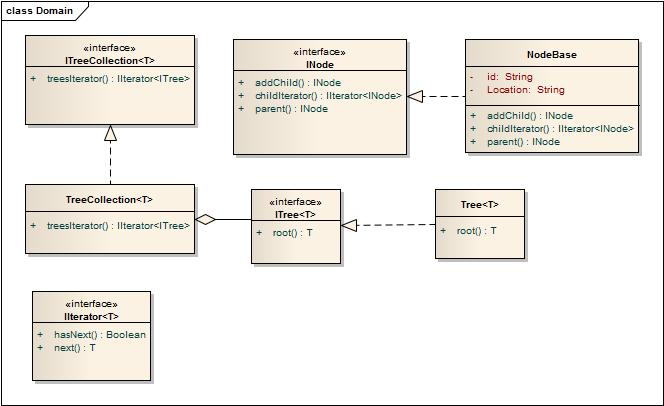
\includegraphics[scale=0.5]{images/Domain.jpg}  
  \caption{UML - Domain}
  \label{uml:Domain}
  \end{figure} 

\subsubsection{DataSource}
\paragraph{}
In Figure~\ref{uml:Domain} is presented a diagram containing the classes for the package DataSource.

  \begin{figure}
  \centering
  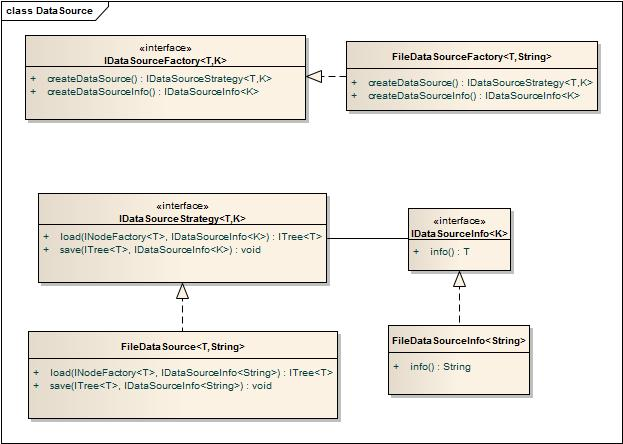
\includegraphics[scale=0.5]{images/DataSource.jpg}  
  \caption{UML - DataSource}
  \label{uml:DataSource}
  \end{figure} 

\subsubsection{Consensor}
\paragraph{}
In Figure~\ref{uml:Consensor} is presented a diagram containing the classes for the package Consensor.

  \begin{figure}
  \centering
  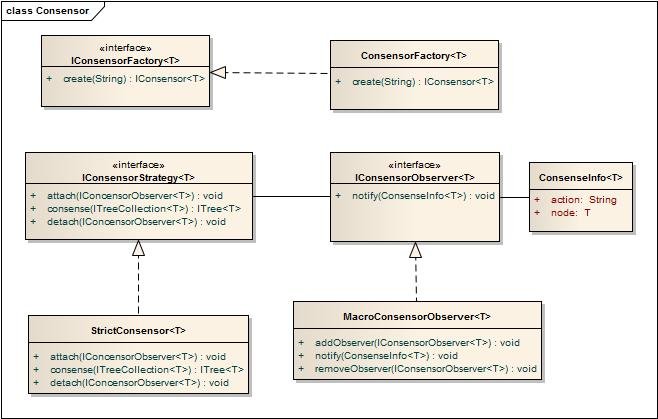
\includegraphics[scale=0.5]{images/Consensor.jpg}  
  \caption{UML - Consensor}
  \label{uml:Consensor}
  \end{figure} 

\subsubsection{Traverser}
\paragraph{}
In Figure~\ref{uml:Traverser} is presented a diagram containing the classes for the package Traverser.

  \begin{figure}
  \centering
  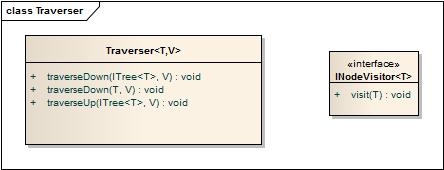
\includegraphics[scale=0.5]{images/Traverser.jpg}  
  \caption{UML - Traverser}
  \label{uml:Traverser}
  \end{figure} 

\subsubsection{Propagator}
\paragraph{}
In Figure~\ref{uml:Propagator} is presented a diagram containing the classes for the package Propagator.

  \begin{figure}
  \centering
  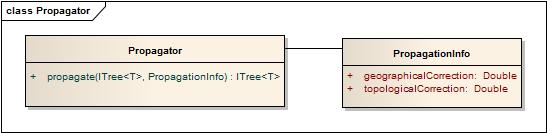
\includegraphics[scale=0.5]{images/Propagator.jpg}  
  \caption{UML - Propagator}
  \label{uml:Propagator}
  \end{figure} 

\subsubsection{Facade}
\paragraph{}
In Figure~\ref{uml:Facade} is presented a diagram containing the classes for the package Facade.

  \begin{figure}
  \centering
  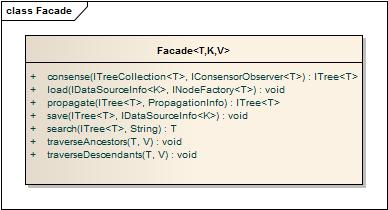
\includegraphics[scale=0.5]{images/Facade.jpg}  
  \caption{UML - Facade}
  \label{uml:Facade}
  \end{figure} 

   
 
 \subsection{Dynamic Diagrams}
 
 \subsubsection{Descendants Selection}
 
   \begin{figure}
  \centering
  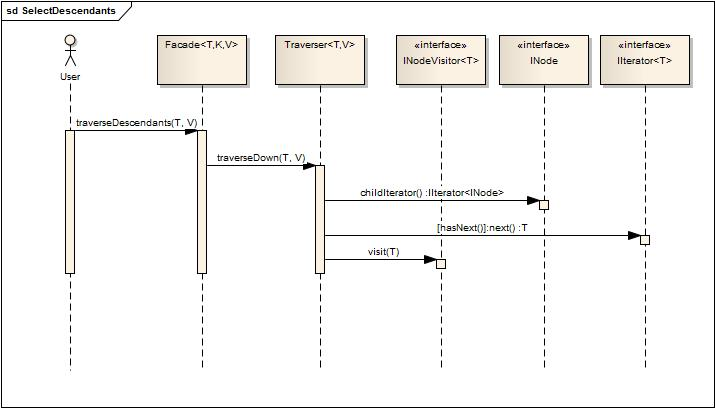
\includegraphics[scale=0.5]{images/SelectDescendants.jpg}  
  \caption{UML - Descendants Selection}
  \label{uml:SelectDescendants}
  \end{figure} 

  
 \subsubsection{Tree Consense}
 
   \begin{figure}
  \centering
  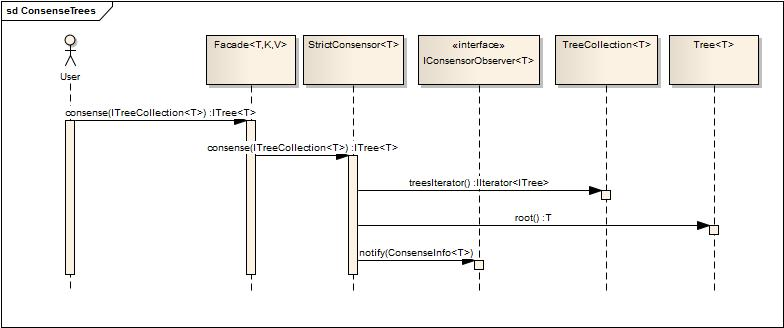
\includegraphics[scale=0.5]{images/ConsenseTrees.jpg}  
  \caption{UML - Tree Consense}
  \label{uml:ConsenseTrees}
  \end{figure} 
  
  
 \subsubsection{Tree Import}
 
   \begin{figure}
  \centering
  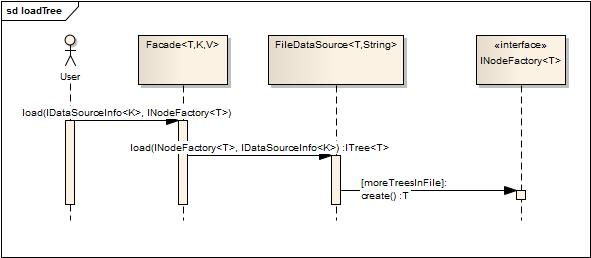
\includegraphics[scale=0.5]{images/loadTree.jpg}  
  \caption{UML - Tree Import}
  \label{uml:loadTree}
  \end{figure} 
  
  
 \subsubsection{Tree Propagation}
 
   \begin{figure}
  \centering
  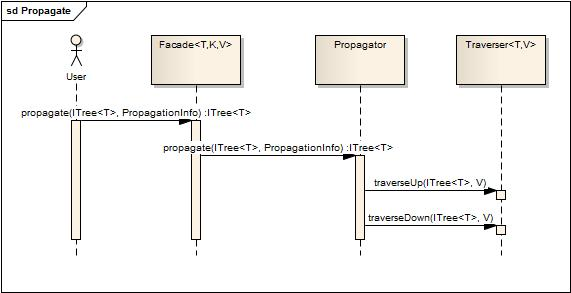
\includegraphics[scale=0.5]{images/Propagate.jpg}  
  \caption{UML - Tree Propagation}
  \label{uml:Propagate}
  \end{figure} 
  
\begin{thebibliography}{9}  
  \bibitem{martin00}
  Design Principles and Design Patterns. Robert C. Martin, 2000.\\
  \url{www.objectmentor.com}
  
    \bibitem{loki}
  Modern C++ Design. Andrei Alexandrescu
  
  \bibitem{bjarne}
  The C++ Programming Languaje. Bjarne Stroustrup.
  
  \bibitem{wirfsbrok03}
  Rebecca Wirfs-Brock and Alan McKean. Object Design: Roles, Responsibilities
and Collaborations, Addison-Wesley, 2003

  \bibitem{uml}
  Unified Modeling Language: \url{http://www.uml.org/}

  \bibitem{argoUML}
  ArgoUML: \url{http://argouml.tigris.org/}

  
\end{thebibliography}
\end{document}


